\noindent 

In this section, we describe a profit-based optimization framework for
the cloud-computing execution model previous described. Using this
framework we compute profit-optimized execution speeds by
optimizing the following objective function:

%It is assumed that failures can be detected.

%While this is the case in many computing
%environments, there are cases where failure detection may not be
%possible. To address this limitation, we propose a sub-optimal shadow
%replication scheme, whereby both the main process and the shadow
%execute independently at stretched speeds to meet the expected
%response time, without the need for the main processes failure
%detection.

%In this section, we describe a reward-based analytical
%model to guide the design of the shadow replication scheme that
%executes at optimal speed to maximize profits. 


%In this section we are going to develop a framework to assess and
%explore the trade-off between energy consumption and performance of
%fault tolerant computation models, namely shadow replication, pure
%replication, and re-execution. To this end, we adopt a reward-based
%model to study the economic potential of shadow replication, analyze its
%interplay between resiliency and power management, and compare it to
%other fault tolerance models.

%Without loss of generality, we focus on the execution of one job as
%shown in Fig. 2, assuming that there are N tasks in total that will
%execute in parallel. The completion of the job depends on the
%successful execution of all these tasks, and a failure in one task
%would delay the completion of the entire job.

\begin{equation}
\label{optimization_problem}
%\setlength{\abovedisplayskip}{14pt}
\begin{alignedat}{2}
\max_{\sigma_m,\sigma_b,\sigma_a}     & E[profit] \\
s.t.                                 & 0 \leq \sigma_m \leq \sigma_{max} \\
                                     & 0 \leq \sigma_b \leq \sigma_{m} \\
                                     & 0 \leq \sigma_a \leq \sigma_{max} 
\end{alignedat}
\end{equation}
We assume that processor
speeds are continuous and use nonlinear optimization techniques
to solve the above optimization problem. 

In order to earn profit, service providers must either increase
income or decrease expenditure. We take both factors into
consideration for the purpose of maximizing profit while meeting
customer's requirements. In our model, we set the expected profit to be
expected income minus expected expense.

\begin{equation}
E[\text{profit}]=E[\text{income}]-E[\text{expense}]
\end{equation}

\subsection{Reward Model}
\label{sla_reward_model}
The cloud computing SLA can be diverse and
complex. To focus on the profit and reliability
aspects of the SLA, we define the reward model based on job completion
time. Platform as a Service (PaaS) companies will continue to become
more popular causing an increase in SLAs using job completion time as
their performance metric. We are already seeing this appear in
web-based remote procedure calls and data analytic requests.

As depicted in Figure \ref{fig:reward}, customers expect that their
job deployed on cloud finishes by a mean response time $t_{R_1}$.  As a
return, the provider earns a certain amount of reward, denoted by R,
for satisfying customer's requirements. However, if the job cannot be
completed by the expected response time, the provider loses a fraction of $R$
proportional to the delay incurred. For large delay, the profit loss may translate into a penalty that the CSP must pay to the customer. In this model, the maximum penalty $P$ is paid if the
delay reaches or exceeds $t_{R_2}$. The four
parameters, $R$, $P$, $t_{R_1}$ and
$t_{R_2}$, completely define the reward model.

%The three parameters, R, and should be determined while negotiating
%the SLA according to the task workload. In our model, R is
%proportional to the expected energy cost that SP has to pay for
%executing customer’s tasks. Especially, R can grow with workload in a
%linearly proportional manner, logarithmic manner, or exponential
%manner.
%
%, which
%should be larger than the minimal response time . 

There are two facts that the service provider must take into account
when negotiating the terms of the SLA. The first is the response time
of the main process assuming no failure (Figure
\ref{fig:sc_no_fail} and Figure \ref{fig:sc_shadow_fail}). This
results in the following completion time:
\begin{equation}
t_c^m=W/\sigma_m
\label{eq:tcm}
\end{equation}

If the main process fails (shown in Figure \ref{fig:sc_main_fail}), the
task completion time by shadow process is the time of the failure,
$t_f$, plus the time necessary to complete the remaining work.

\begin{equation}
t_c^s=t_f+\frac{W-t_f \times \sigma_b}{\sigma_a}
\label{eq:tcs}
\end{equation}

This reward model is flexible and extensible; it is not restricted to
the form shown in Figure \ref{fig:reward}. In particular, the decrease
may be linear, concave, or convex and the penalty can extend to
infinity. This model can further be extended to take into
consideration both the short-term income and long-term reputation of
the service provider~\cite{Daw:2002:LRP:639717.639720}.


\begin{figure}[t!]	
	\begin{center}
		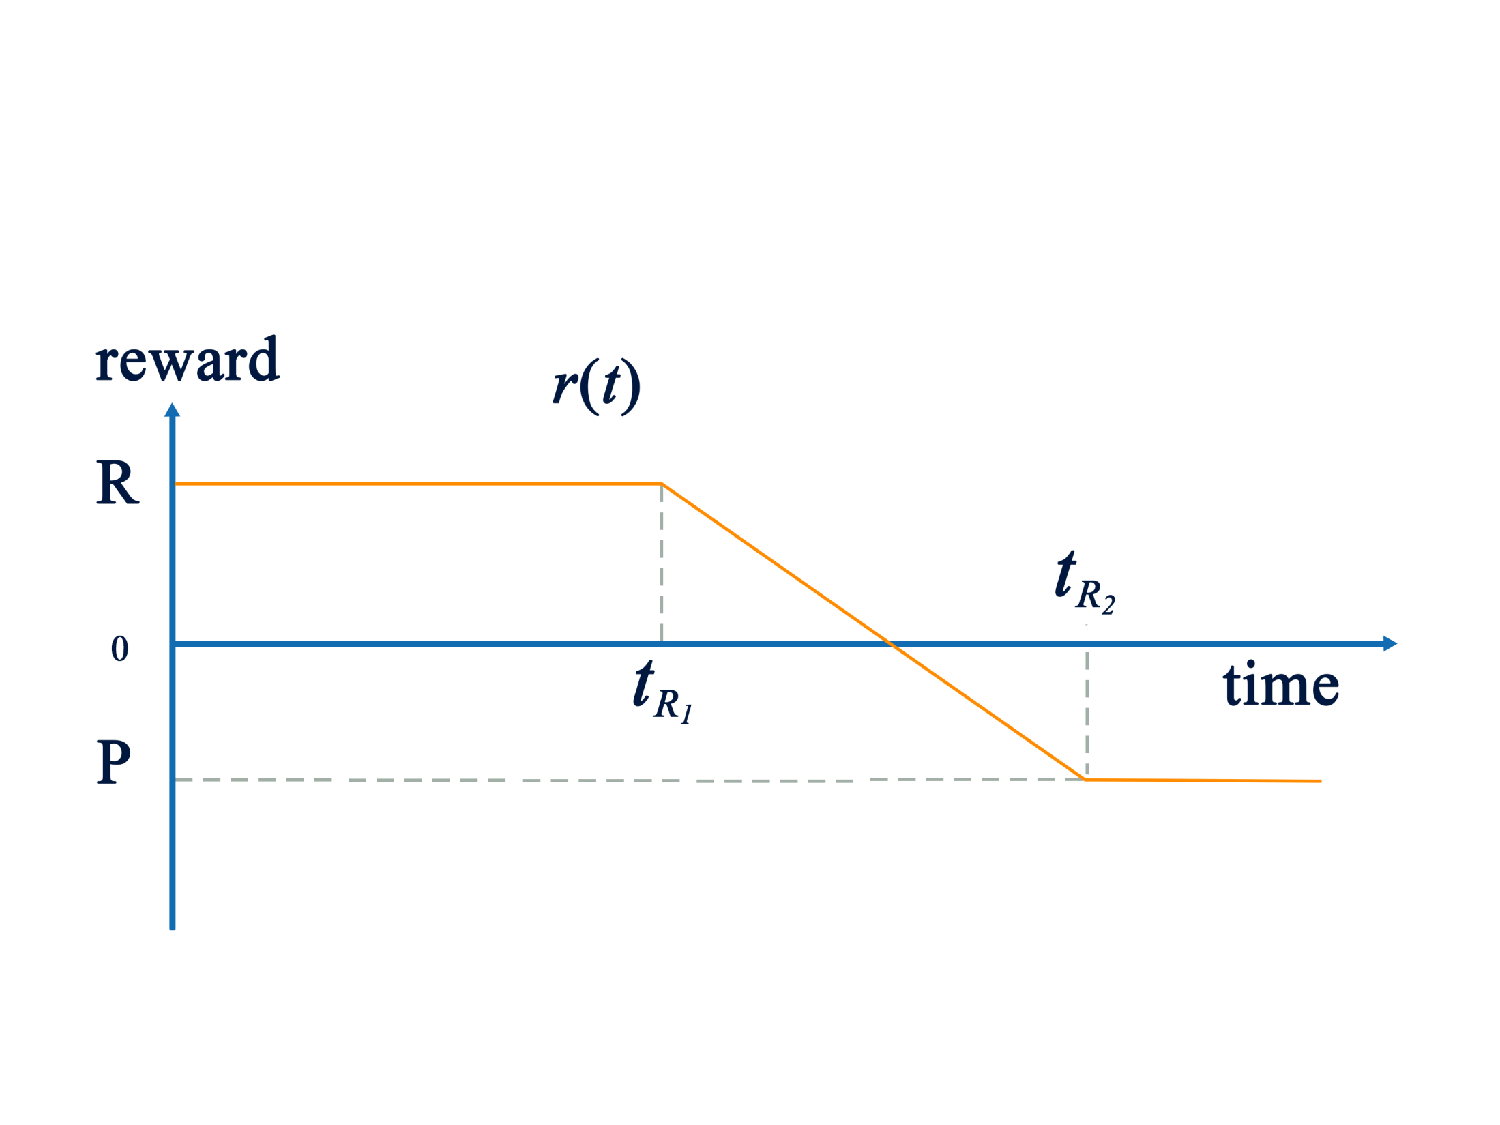
\includegraphics[width=\columnwidth]{diagrams/reward.pdf}
	\end{center}
	\caption{A reward function}
	\label{fig:reward}
\end{figure}


\subsection{Failure Model}
Failure can occur at any point during the execution of the main or
shadow process. Our assumption is that at most one failure occurs,
therefore if the main process fails it is implied that the shadow will
complete the task without failure. We can make this assumption because
we know the failure of any one node is rare thus the failure
of any two specific nodes is very unlikely.

% I don't think we need to say this and it opens us up to having to
% explain multiple shadows which we do not do today.
%In order
%to achieve higher resiliency one would make use of multiple shadow
%processes and this failure model will still be valid.

We assume that two probability density functions, $f_m(t_f)$ and
$f_s(t_f)$, exist which express the probabilities of the main and shadow
process failing at time $t_f$ separately. The model does not assume a
specific distribution. However, in the remainder of this paper we use
an exponential probability density function, $f_m(t_f)=f_s(t_f)=\lambda
e^{-\lambda t_f}$, of which the mean time between failure (MTBF) is $\frac{1}{\lambda}$.

\subsection{Power and Energy Models}
Dynamic voltage and frequency scaling
(DVFS) has
been widely exploited as a technique to reduce CPU dynamic power~\cite{flautner_2002_APS,pillai_2001_sosp}. It
is well known that one can reduce the dynamic CPU power consumption at
least quadratically by reducing the execution speed linearly. The
dynamic CPU power consumption of a computing node executing at speed
$\sigma$ is given by the function $p_d(\sigma)=\sigma^n$ where $n \ge
2$.
%% removed burd_1995_systems citation

In addition to the dynamic power, CPU leakage and other components
(memory, disk, network etc.) all contribute to static power
consumption, which is independent of the CPU speed. In this paper we
define static power as a fixed fraction of the node power consumed
when executing at maximum speed, referred to as $\rho$. Hence node
power consumption is expressed as
$p(\sigma)=\rho \times \sigma_{max}^n + (1-\rho)\times \sigma^n$. When the execution speed is zero
the machine is in a sleep state, powered off or not assigned as a
resource; therefore it will not be consuming any power, static or
dynamic.  Throughout this paper we assume that dynamic power is cubic
in relation to
speed~\cite{rusu_2003_ecs,zhai_2004_dac}, therefore the
overall system power when executing at speed $\sigma$ is defined as:
\begin{equation}
p(\sigma) = \begin{cases} \rho \sigma_{max}^3 + (1-\rho) \sigma^3 & \mbox{if } \sigma > 0 \\ 
                          0 & \mbox{if } \sigma = 0 \end{cases}
\label{eq:power_model}
\end{equation}
%% I removed chen_2012_srds from speed citation to save space

Using the power model given by \refeq{eq:power_model}, the
energy consumed by a process executing at speed $\sigma$ during an
interval $T$ is given by
\begin{equation}
E(\sigma,T) = p(\sigma) \times T
\end{equation}

%We derive the expected energy consumption of shadow replication for a
%single task assuming the failure model described
%previously. 

Corresponding to \reffig{fig:sc_overview}, there are three
failure cases to consider: main and shadow both succeed, shadow fails
and main fails. As described earlier, the case of both the main and
shadow failing is very rare and will be ignored. The expected
energy consumption for a single task is then the weighted average of
the expected energy consumption in the three cases.

%Each task is dependent upon the completion of all other tasks, this
%means that if a task completes prior to another task it must idly wait
%for that task to complete. In our system model a task will have to
%wait if at least one main process fails to complete, thus forcing all
%tasks to wait until the latest shadow process completes. 

First consider the case where no failure occurs and the main process
successfully completes the task at time $t_c^m$, corresponding to
\reffig{fig:sc_no_fail}.
\begin{equation}
\begin{split}
E_1 = &  ( 1-\int_0^{t_c^m}f_m(t)dt) \times (1 - \int_0^{t_c^m} f_s(t)dt) \times \\
      &  (  E(\sigma_m,t_c^m) + E(\sigma_b,t_c^m))
\label{eq:energy_no_failure}
\end{split}
\end{equation}
The first line is the probability of fault-free execution of the main
process and shadow process. Then we multiple this probablity by the
energy consumed by the main and the shadow process during this fault
free execution, ending at $t_c^m$.

Next, consider the case where the shadow process fails at some point
before the main process successfully completes the task, corresponding to
\reffig{fig:sc_shadow_fail}.
\begin{equation}
\begin{split}
E_2 = & (1-\int_0^{t_c^m}f_m(t)dt) \times \\
      & \int_0^{t_c^m}(E(\sigma_m,t_c^m)+E(\sigma_b,t)) \times f_s(t)dt
\label{eq:energy_shadow_fail}
\end{split}
\end{equation}
The first factor is the probability that the main process does not
fail, and the probability of shadow fails is included in the second factor which also contains the energy consumption since it depends on the shadow failure time. Energy consumption comes from the main process until the completion of the task,
and the shadow process before its failure.

The one remaining case to consider is when the main process fails and
the shadow process must continue to process until the task completes,
corresponding to Figure \ref{fig:sc_main_fail}.
\begin{equation}
\begin{split}
E_3 = & (1-\int_0^{t_c^m}f_s(t)dt) \times \int_0^{t_c^m}(E(\sigma_m,t)+\\
      & E(\sigma_b,t)+E(\sigma_a,t_c^s-t))f_m(t)dt
\label{eq:energy_main_fail}
\end{split}
\end{equation}
Similarly, the first factor expresses the probability that the shadow process does
not fail. In this case, the shadow process executes from the beginning to
$t_c^s$ when it completes the task. However, under our ``at most one
failure'' assumption, the period during which shadow process may fail
ends at $t_c^m$, since the only reason why shadow process is still in
execution after $t_c^m$ is that main process has already failed. There
are three parts of energy consumption, including that of main process
before main's failure, that of shadow process before main's failure,
and that of shadow process after main's failure, all of which depend
on the failure occurrence time. 

The three equations above describe the expected energy consumption by a
pair of main and shadow processes for completing a task under
different situations. However, under our system model it might be the
case that those processes that finish early will wait idly and
consume static power if failure delays one task. If it is the case
that processes must wait for all tasks to complete, then this energy
needs to be accounted for in our model. The probability of this is the probability that at least one main process fails,
referred to as the system level failure probability.
\begin{equation}
P_f=1-(1-\int_0^{t_c^m}f_m(t)dt)^N
\label{eq:prob_of_one_main_failure}
\end{equation}
Hence, we have the fourth equation corresponding to the energy consumed while waiting in idle. 
\begin{equation}
  \begin{split}
  E_4 = & ( 1-\int_0^{t_c^m}f_m(t)dt) \times (1 - \int_0^{t_c^m} f_s(t)dt) \times \\
        & 2 P_f \times E(0,t_c^j-t_c^m) + \int_0^{t_c^m}f_s(t)dt \times \\
        & (1-\int_0^{t_c^m}f_m(t)dt) \times P_f \times E(0,t_c^j-t_c^m) 
  \end{split}
\end{equation}
Corresponding to the first case, neither main process nor shadow
process fails, but both of them have to wait in idle from task
completion time $t_c^m$ to the last task's completion (by a shadow
process) with probability $P_f$. Under the second case, only the main
process has to wait if some other task is delayed since its shadow
process has already failed. These two aspects are accounted in the
first and last two lines in $E_4$ separately.  We use the expected
shadow completion time $t_c^j$ as an approximation of the latest task
completion time which is also the job completion time.

%% Rami said remove, I agree - bnm
%and the reason why we
%ignore the third case is that the third case itself accounts for the
%delayed task and it is already factored in $E_3$. 

%\begin{equation}
%t_c^j=\frac{\int_0^{t_c^m}t_c^s \times f_m(t)dt}{\int_0^{t_c^m}f_m(t)dt}
%\label{eq:estimated_shadow_completion}
%\end{equation}

By summing these four parts and then multiplying it by $N$ we will have
the expected energy consumed by Shadow Replication for completing a
job of $N$ tasks.
\begin{equation}
E[\text{energy}]=N \times (E_1 + E_2 + E_3 + E_4)
\label{eq:total_energy}
\end{equation}

\subsection{Income and Expense Models}
The income is the reward paid by customer for the cloud computing
services that they utilize. It depends on the reward function $r(t)$,
depicted in \reffig{fig:reward}, and the actual job completion
time. Therefore, the income should be either $r(t_c^m)$, if all main
processes can complete without failure, or $r^*(t_c^s)$ otherwise. It
is worth noting that the reward in case of failure should be
calculated based on the last completed task, which we approximate by
calculating the expected time of completion allowing us to derive the
expected reward, i.e. $r^*(t_c^s)=\frac{\int_0^{t_c^m}r(t_c^s) \times
f_m(t)dt}{\int_0^{t_c^m}f_m(t)dt}$. Therefore the income is estimated
by the following equation.
\begin{equation}
E[\text{income}]= (1-P_f) \times r(t_c^m) + P_f \times r^*(t_c^s)
\end{equation}

%% there is some hand-waving maddness above, unclear how to fix? -bnm

The first part is the reward earned by the main process times the
probability that all main processes would complete tasks without
failure. If at least one main process fails, that task would have to
be completed by a shadow process. As a result, the second part is the
reward earned by shadow process times the system level failure probability.

If $C$ is the charge expressed as dollars per unit of energy consumption
(e.g. kilowatt hour), then the expected expenditure would be $C$ times
the expected energy consumption for all $N$ tasks:
\begin{equation}
E[\text{expense}] = C \times E[\text{energy}]
\label{eq:expense}
\end{equation}

However, the expenditure of running the cloud computing service is more
than just energy, and must includes hardware, maintenance, and human
labor. These costs can be accounted for by amortizing these costs into the
static power factor, $\rho$. Because previous studies have
suggested~\cite{Elnozahy03energyconservation,Raghavendra:2008:NPS}
that energy will become a dominate factor we decided to focus on this
challenge and leave other aspects to future work.

\begin{table}[!h]
\caption{Symbols used in our analytical model.}
\centering
\begin{tabularx}{\columnwidth}{|l|X|}
\hline
Symbols                          & Definition                         \\
\hline
$W$                               & Task size                       \\
\hline
$N$                               & Number of tasks                 \\
\hline
$r(t)$                          & Reward function       \\
\hline
$R$, $P$                            & Maximum reward and penalty      \\
\hline
$t_{R_1}$, $t_{R_2}$             & Response time thresholds  \\
\hline
$C$                               & Unit price of energy            \\
\hline
$\rho$                          & Static power ratio                 \\
\hline
$t_c^m$, $t_c^s$, $t_c^{j}$                 & Completion time of main process, shadow process, and the whole job \\
\hline
$f_m()$, $f_s()$                    & Failure density function of main and shadow  \\
\hline
$\lambda$                           & Failure rate    \\
\hline
$P_f$                               & System level failure probability \\
\hline
$\sigma_m$, $\sigma_b$, $ \sigma_a$  & Speeds of main, shadow before and after failure (Optimization Outputs) \\
\hline
\end{tabularx}

\label{tbl:symbols}
\end{table}

Based on the above formalization of the optimization problem, the
MATLAB Optimization Toolbox~\cite{matlab_opt} was used to solve the
resulting nonlinear optimization problem. The parameters of this
problem are listed in Table~\ref{tbl:symbols}. 



